\documentclass[11pt,openright,twoside]{report}
\usepackage[utf8]{inputenc}
\usepackage[hmargin=4cm,vmargin=3.5cm,bmargin=3.5cm]{geometry}
\usepackage[portuguese, english]{babel}
\usepackage{graphicx}
\usepackage{hyperref}
\usepackage{natbib}
\usepackage{indentfirst}
\renewcommand{\rmdefault}{phv}
\renewcommand{\sfdefault}{phv}
\renewcommand{\baselinestretch}{1.1}


\title{\textbf{Relatório - HTML}}

\begin{document}

\begin{titlepage}
\begin{figure}
\title{\textbf{Relatório - HTML}}
\author{P1 - Rúben Paulo Cunha Pequeno\\
P3 - Marta Cristina Ferreira Coutinho de Almeida\\\
P5 - Rui Pereira de Melo Silva de Albuquerque\\
P4 - António Miguel Fonseca Rebelo Pereira\\\vspace{3cm}
Universidade de Aveiro - Laboratórios de Informática}
\date{\today}
 
\includegraphics[scale=0.9]{ua_logo.png}
\end{figure}
\end{titlepage}

\selectlanguage{portuguese}
\maketitle
\tableofcontents
\listoffigures

\part{Apresentação}

\chapter{Resumo}
Neste relatório iremos fazer uma análise detalhada ao código-fonte HTML de uma página Web com recurso a bases de dados, que nos foi proposto realizar na UC Laboratórios de Informática. Ao longo do relatório iremos explicar cada página detalhadamente com recurso a algumas imagens.
\smallskip


\chapter{Introdução}
HTML é um linguagem de marcação de hipertexto \cite{markup}, desenvolvida na década de 1980 por Tim Beerners-Lee \cite{HTML}, físico britânico que na época trabalhava no \textit{CERN} \cite{CERN}. Esta ferramenta surgiu para facilitar a partilha de arquivos entre engenheiros e físicos no seu local de trabalho. No entanto, só no início de 1990 foi desenvolvido um browser capaz de a ler. É uma linguagem baseada em SGML \cite{SGML} e HyTime \cite{HyTime}, ambas linguagens de marcação de hipertexto (\autoref{estruhtml}).
\smallskip

\begin{figure}
 \center
 
\includegraphics[scale=0.35]{HTML.jpg}
 \caption{Estrutura ilustrativa de um código HTML.}
 \label{estruhtml}
\end{figure}

Desde 1995, com o crescimento e o desenvolvimento da Internet \cite{Internetus}, a linguagem tornou-se muito popular pot todo o mundo, nomeadamente pela sua simplicidade e robustez. Ao longo dos anos, foi também recebendo algumas adições de outras linguagens para completar a sua implementação em páginas \textit{Web}. As principais linguagens de programação implementadas em parceria com HTML são Javascript \cite{Javascript} e CSS \cite{Css}. A linguagem tem sido bastante otimizada, contendo já várias versões durante o seu aperfeiçoamento, sendo a mais recente a versão 5.0 \citep{w3c} (\autoref{estruhtml}).
\smallskip 


Bancos de dados são conjuntos de repositórios relacionados entre si que contêm registos de pessoas, sítios ou objetos. São conjuntos de dados planificados que estão logicamente interligados e fornecem eficiência adicional durante a pesquisa.
\smallskip

Pretendemos, portanto, explorar a linguagem HTML com recurso a bases de dados. Vamos, então, anlisar uma página que faz uso de um sistema de Logins. O código-fonte criado é providenciado na pasta "html", com o nome \textit{"index.htm"}% (\url{})

\part{Desenvolvimento}

\chapter{Apresentação das páginas web}
Nesta secção vai ser explicada o atual funcionamento do website/app. Apenas as páginas de Login/Registo de novo utilizador foram criadas, assim como a página do acerca(about).
\smallskip

\section{Login Page}
\begin{figure}
 \center
 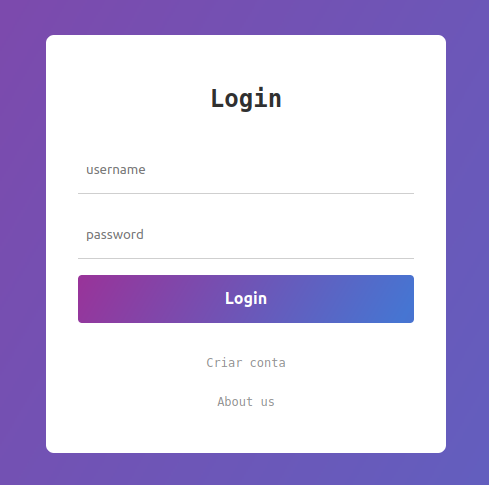
\includegraphics[scale=.25]{Login.png}
 \caption{Página de Login.}
 \label{bse}
\end{figure}

Na primeira página(/ ou /index), ao tentar fazer login, a função users/auth vai verificar primeiro, se o username existe e de seguida irá verificar se a password introduzida corresponde à guardada na base de dados. No final esta função devolve um json tal com as keys: "authentication", "token" e "error", dizendo se a autenticação falhou ou passou, dando um token caso seja aprovada(não funcional) e uma mensagem de erro.
\smallskip

\section{New User page}
\begin{figure}
 \center
 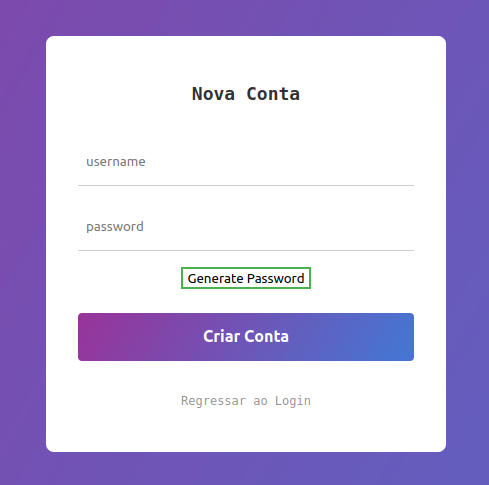
\includegraphics[scale=.25]{NovaConta.png}
 \caption{Página de Criaçao de Conta.}
 \label{bse}
\end{figure}

Se clicar-mos em "Criar Conta", o site será redirecionado para a página de criação de um novo usuário(/newUser) na qual poderá criar uma nova conta, adicionando-a assim à base de dados já existente. Neste caso, a função users/create irá verificar se já existe o username selecionado, caso não haja, irá guardar o username e password na base de dados. Esta função também devolve um json com as keys "create" e "error" a dizer se foi criado com sucesso ou devolvendo uma mensagem de erro. Também tem um botão que gera uma password random feito em javascript(falta botão pôr a password visivel). Finalmente tem a opção de voltar para o menu de login.
\smallskip

\section{About page}
\begin{figure}
 \center
 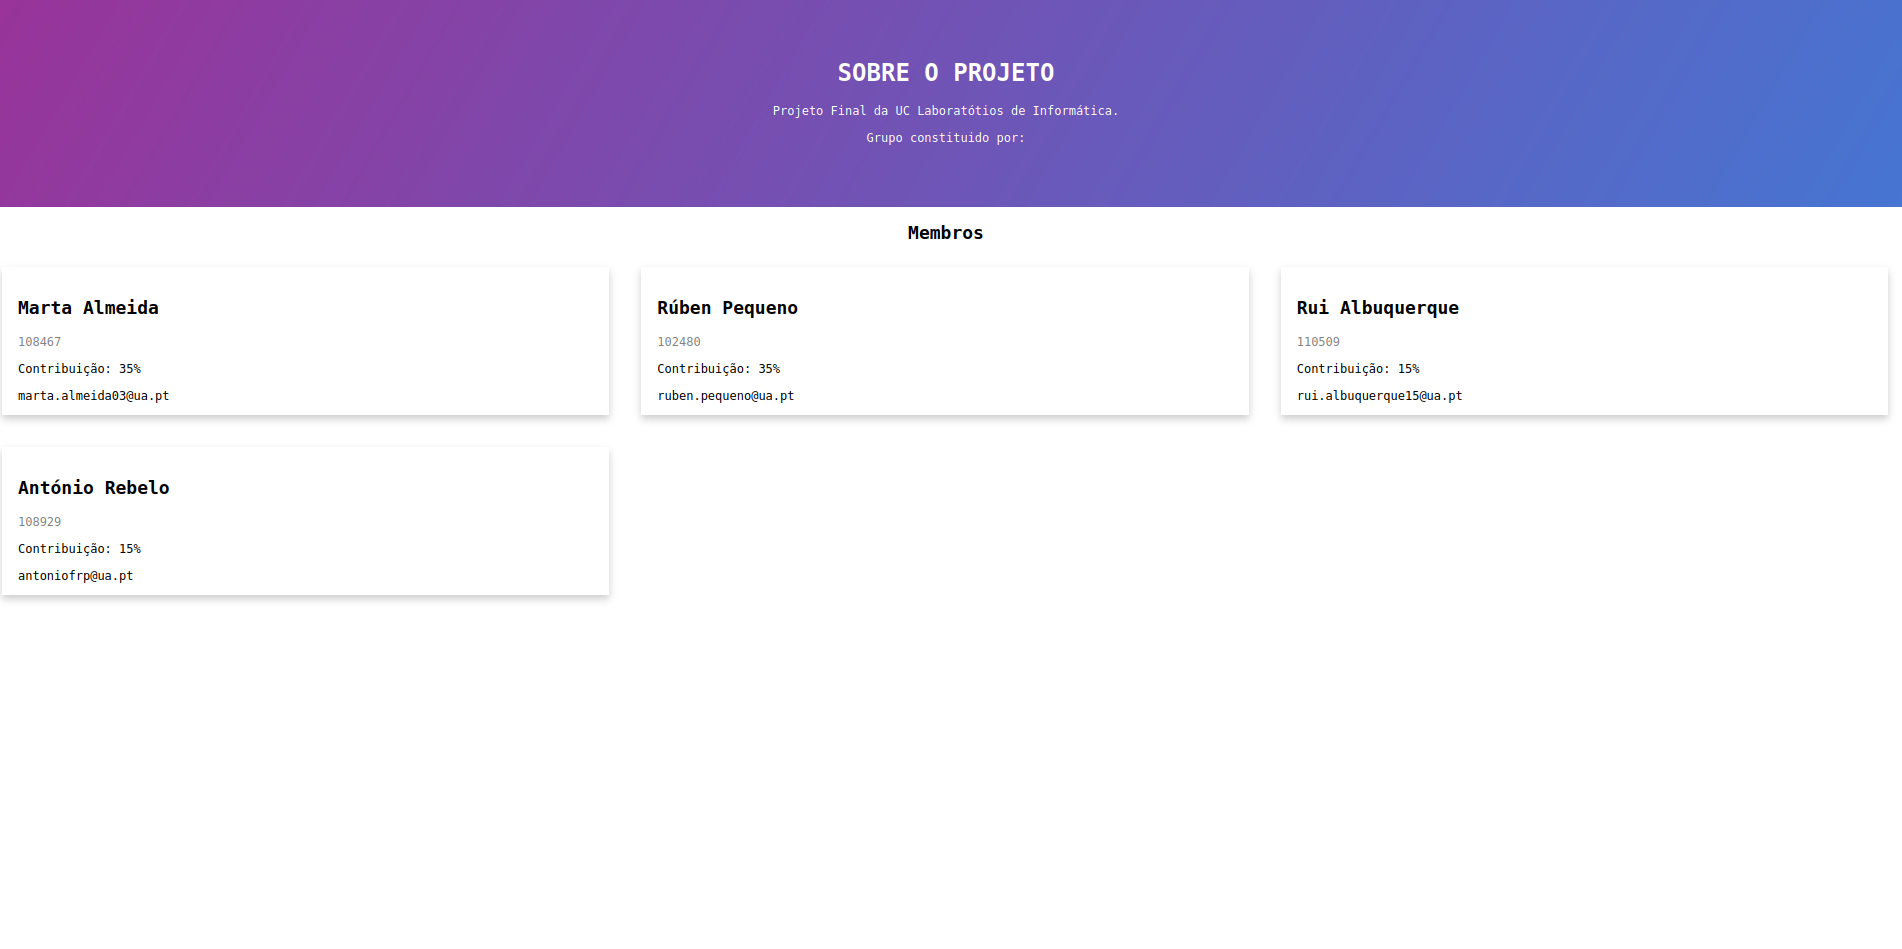
\includegraphics[scale=.25]{about.png}
 \caption{Página de About.}
 \label{bse}
\end{figure}

Finalmente, na página de login tem o link de acesso ("About Us") para ir para a página do acerca, onde podemos encontrar as informações dos membros do grupo.
\smallskip

\part{Conclusão}

\chapter{Conclusão}
Considerando, o estudo da linguagem HTML e de bases de dados, após a concretização deste relatório podemos dizer que é uma linguagem bastante indispensável na criação e desenvolvimento de páginas web dinâmicas. Apartir uma análise detalhada e a elaboração de uma página dinâmica, foi possível abordar uma grande quantidade de aspetos essenciais e compreender o funcionamento de páginas web dinâmicas.
\smallskip

Concluímos, que é trabalhar com páginas dinâmicas tem a sua complexidade e que ao longo do nosso projeto encontramos certos desafios que não consguimos concluir na sua totalidade, mas com certeza o Projeto realizar o projeto ajudou-nos a entender melhor o uso de bases de dados, asism como fazer manipulação de imagem num site.
\smallskip

Para finalizar, acrescentamos que a moiria do trabalho foi realizado pelo Rúben Pequeno (35\%) e Marta Almeida (35\%), o restante foi realizado pelo Rui Albuquerque (15\%) e António Rebebelo (15\%).

\bibliography{bibe}
\bibliographystyle{plain}


\end{document}
